
%(BEGIN_QUESTION)
% Copyright 2006, Tony R. Kuphaldt, released under the Creative Commons Attribution License (v 1.0)
% This means you may do almost anything with this work of mine, so long as you give me proper credit

Forklar hvordan man kan øke integraltiden (antall minutter per repetisjon) i denne pneumatiske regulatoren:

$$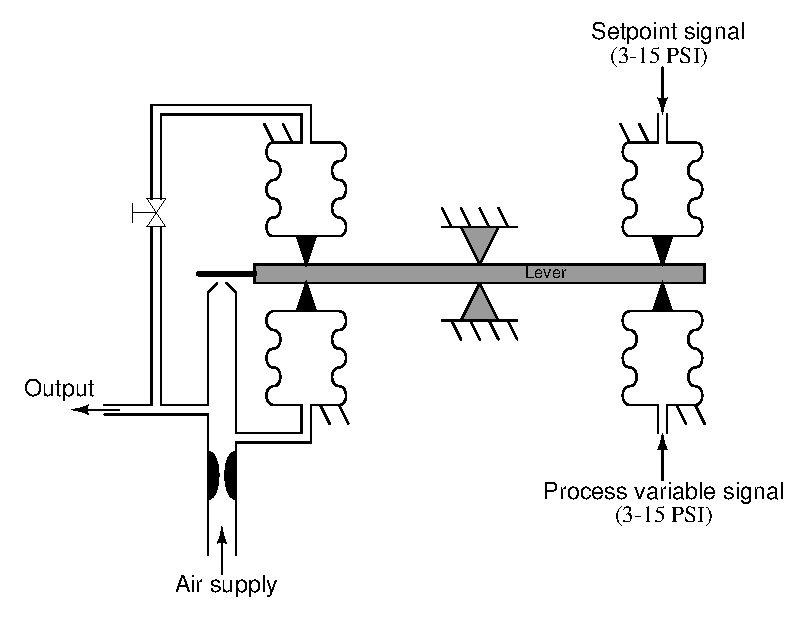
\includegraphics[width=15.5cm]{i01598x01.eps}$$

Bestem også om dette er en {\it proporsjonal + integral} (PI)-regulator eller en {\it kun integral} (I)-regulator, og forklar begrunnelsen din.

\vskip 20pt \vbox{\hrule \hbox{\strut \vrule{} {\bf Forslag til sokratisk diskusjon} \vrule} \hrule}

\begin{itemize}
\item{} Hvordan ville du endret mekanismen for motsatt virkemåte (for eksempel direkte versus revers)?
\item{} Forklar hvordan mekanismen ville reagert på et avvik (PV $-$ SP) hvis strupeventilen var plassert i serie med nedre venstre belg i stedet for øvre venstre belg, slik som vist.
\item{} Anta at både utgangsbelgen og reset-belgen ble byttet med belger med samme areal, men større volum (altså {\it lengre} belger). Hvilken effekt ville dette hatt på regulatorens {\it forsterkning} og på regulatorens {\it integraltidskonstant}?
\item{} Anta at både utgangsbelgen og reset-belgen ble byttet med bredere belger som både hadde større areal og større volum. Hvilken effekt ville dette hatt på regulatorens {\it forsterkning} og på regulatorens {\it integraltidskonstant}?
\item{} Er det mulig å justere regulatorens forsterkning uten å påvirke integraltidskonstanten, ved å endre bare én del av mekanismen (for eksempel flytte en belg, flytte vippepunktet osv.)? Forklar hvorfor eller hvorfor ikke.
\item{} Merk at denne pneumatiske regulatoren mangler {\it bias-fjæren} som finnes i P-regulatorer. Forklar hvorfor.
\item{} Anta at vanndamp i trykkluftforsyningen kondenserer til flytende vann og samler seg i bunnen av reset-belgen. Hvilken effekt kan dette ha på regulatorens ytelse, om noen?
\end{itemize}

\underbar{file i01598}
%(END_QUESTION)





%(BEGIN_ANSWER)

Strup ventilen mer for å øke $\tau_i$ i denne PI-regulatoren.

%(END_ANSWER)





%(BEGIN_NOTES)

Når ventilen strupes, reduseres luftstrømmen inn i eller ut av øvre belg for et gitt avvik mellom PV og SP, og dermed endres utgangstrykket saktere over tid.

\vskip 10pt

Vi kan avgjøre hvilke reguleringsmåter en regulator har ved å se responsen på en plutselig påført endring (et ``trinn'') i avviket (PV $-$ SP). Utgangssignalet til en regulator med kun integralvirkning vil bare begynne å rampe når et slikt avvik oppstår. Utgangssignalet til en regulator med proporsjonal + integralvirkning vil først ``hoppe'' som respons på det plutselige avviket, {\it deretter} rampe med en hastighet bestemt av avvikets størrelse.

Siden utgangssignalet til denne pneumatiske regulatoren ``hopper'' umiddelbart når avviket påføres, vet vi at den har proporsjonalvirkning i tillegg til integralvirkning. Dermed er dette en PI- eller P+I-regulator. Det er {\it ikke} en regulator med kun integralvirkning (``floating response'').

%INDEX% Control, proportional + integral: pneumatic force-balance controller

%(END_NOTES)
